%-----------------------------------------------------------------------------
%
%               Template for sigplanconf LaTeX Class
%
% Name:         sigplanconf-template.tex
%
% Purpose:      A template for sigplanconf.cls, which is a LaTeX 2e class
%               file for SIGPLAN conference proceedings.
%
% Guide:        Refer to "Author's Guide to the ACM SIGPLAN Class,"
%               sigplanconf-guide.pdf
%
% Author:       Paul C. Anagnostopoulos
%               Windfall Software
%               978 371-2316
%               paul@windfall.com
%
% Created:      15 February 2005
%
%-----------------------------------------------------------------------------


% \documentclass[preprint,nonatbib]{sigplanconf}
\documentclass[a4paper, 11pt]{article}

% The following \documentclass options may be useful:

% preprint       Remove this option only once the paper is in final form.
%  9pt           Set paper in  9-point type (instead of default 10-point)
% 11pt           Set paper in 11-point type (instead of default 10-point).
% numbers        Produce numeric citations with natbib (instead of default author/year).
% authorversion  Prepare an author version, with appropriate copyright-space text.
 
\usepackage{amsmath}

\newcommand{\cL}{{\cal L}}

\usepackage{xspace}
\usepackage{graphicx}

\usepackage{ifthen}
\usepackage{alltt}

\usepackage{amsthm}

\usepackage[export]{adjustbox} %For images
\usepackage{float} 

% \theoremstyle{plain}
% \newtheorem{thm}{Theorem}[chapter] % reset theorem numbering for each chapter
\theoremstyle{definition}
\newtheorem{defn}{Definition} % definition numbers are dependent on theorem numbers
% \newtheorem{exmp}[thm]{Example} % same for example numbers



\usepackage{xcolor}
\usepackage{amsmath}
\usepackage{amssymb}
\newboolean{showcomments}
\setboolean{showcomments}{true}
\ifthenelse{\boolean{showcomments}}
  {\newcommand{\bnote}[2]{
	\fbox{\bfseries\sffamily\scriptsize#1}
    {\sf\small$\blacktriangleright$\textit{#2}$\blacktriangleleft$}
    % \marginpar{\fbox{\bfseries\sffamily#1}}
   }
   \newcommand{\cvsversion}{\emph{\scriptsize$-$Id: macros.tex,v 1.1.1.1 2007/02/28 13:43:36 bergel Exp $-$}}
  }
  {\newcommand{\bnote}[2]{}
   \newcommand{\cvsversion}{}
  } 


\newcommand{\here}{\bnote{***}{CONTINUE HERE}}
\newcommand{\nb}[1]{\bnote{NB}{#1}}

\newcommand{\fix}[1]{\bnote{FIX}{#1}}
%%%% add your own macros 

\newcommand{\ab}[1]{\bnote{Alex}{#1}}
\newcommand{\sd}[1]{\bnote{Stef}{#1}}
\newcommand{\ja}[1]{\bnote{Jannik}{#1}}
\newcommand{\md}[1]{\bnote{MD}{#1}}
\newcommand{\jr}[1]{\bnote{JRe}{#1}}
\newcommand{\lf}[1]{\bnote{Luc}{#1}}
\newcommand{\spb}[1]{\bnote{Santi}{#1}}
\newcommand{\td}[1]{\bnote{Thomas}{#1}}
\newcommand{\gp}[1]{\bnote{Guille}{#1}} %% HAHA I GOT HEREEE
\graphicspath{{figures/}}
%%% 


\newcommand{\figref}[1]{Figure~\ref{fig:#1}}
\newcommand{\figlabel}[1]{\label{fig:#1}}
\newcommand{\tabref}[1]{Table~\ref{tab:#1}}
\newcommand{\layout}[1]{#1}
\newcommand{\commented}[1]{}
\newcommand{\secref}[1]{Section \ref{sec:#1}}
\newcommand{\seclabel}[1]{\label{sec:#1}}

%\newcommand{\ct}[1]{\textsf{#1}}
\newcommand{\stCode}[1]{\textsf{#1}}
\newcommand{\stMethod}[1]{\textsf{#1}}
\newcommand{\sep}{\texttt{>>}\xspace}
\newcommand{\stAssoc}{\texttt{->}\xspace}

\newcommand{\stBar}{$\mid$}
\newcommand{\stSelector}{$\gg$}
\newcommand{\ret}{\^{}}
\newcommand{\msup}{$>$}
%\newcommand{\ret}{$\uparrow$\xspace}

\newcommand{\myparagraph}[1]{\noindent\textbf{#1.}}
\newcommand{\eg}{\emph{e.g.,}\xspace}
\newcommand{\ie}{\emph{i.e.,}\xspace}
\newcommand{\etal}{\emph{et al.,}\xspace}
\newcommand{\ct}[1]{{\textsf{#1}}\xspace}


% \newenvironment{code}
%     {\begin{alltt}\sffamily}
%     {\end{alltt}\normalsize}

\newcommand{\defaultScale}{0.55}
\newcommand{\pic}[3]{
   \begin{figure}[h]
   \begin{center}
   \includegraphics[scale=\defaultScale]{#1}
   \caption{#2}
   \label{#3}
   \end{center}
   \end{figure}
}

\newcommand{\twocolumnpic}[3]{
   \begin{figure*}[!ht]
   \begin{center}
   \includegraphics[scale=\defaultScale]{#1}
   \caption{#2}
   \label{#3}
   \end{center}
   \end{figure*}}

\newcommand{\infe}{$<$}
\newcommand{\supe}{$\rightarrow$\xspace}
\newcommand{\di}{$\gg$\xspace}
\newcommand{\adhoc}{\textit{ad-hoc}\xspace}

\usepackage{url}            
\makeatletter
\def\url@leostyle{%
  \@ifundefined{selectfont}{\def\UrlFont{\sf}}{\def\UrlFont{\small\sffamily}}}
\makeatother
% Now actually use the newly defined style.
\urlstyle{leo}

% For Smalltalk source code START
\usepackage{color}
\usepackage{textcomp}
\usepackage{listings}
 
\definecolor{source}{gray}{0.85}% my comment style
\newcommand{\myCommentStyle}[1]{{\footnotesize\sffamily\color{gray!100!white} #1}}
%\newcommand{\myCommentStyle}[1]{{\footnotesize\sffamily\color{black!100!white} #1}}
 
% my string style
\newcommand{\myStringStyle}[1]{{\footnotesize\sffamily\color{violet!100!black} #1}}
%\newcommand{\myStringStyle}[1]{{\footnotesize\sffamily\color{black!100!black} #1}}
 
% my symbol style
\newcommand{\mySymbolStyle}[1]{{\footnotesize\sffamily\color{violet!100!black} #1}}
%\newcommand{\mySymbolStyle}[1]{{\footnotesize\sffamily\color{black!100!black} #1}}
 
% my keyword style
\newcommand{\myKeywordStyle}[1]{{\footnotesize\sffamily\color{green!70!black} #1}}
%\newcommand{\myKeywordStyle}[1]{{\footnotesize\sffamily\color{black!70!black} #1}}
 
% my global style
\newcommand{\myGlobalStyle}[1]{{\footnotesize\sffamily\color{blue!100!black} #1}}
%\newcommand{\myGlobalStyle}[1]{{\footnotesize\sffamily\color{black!100!black} #1}}
 
% my number style
\newcommand{\myNumberStyle}[1]{{\footnotesize\sffamily\color{brown!100!black} #1}}
%\newcommand{\myNumberStyle}[1]{{\footnotesize\sffamily\color{black!100!black} #1}}
 
\lstset{
language={},
% characters
tabsize=3,
escapechar={!},
keepspaces=true,
breaklines=true,
alsoletter={\#},
literate={\$}{{{\$}}}1,
breakautoindent=true,
columns=fullflexible,
showstringspaces=false,
% background
frame=single,
aboveskip=1em, % automatic space before
framerule=0pt,
basicstyle=\footnotesize\sffamily\color{black},
keywordstyle=\myKeywordStyle,% keyword style
commentstyle=\myCommentStyle,% comment style
frame=single,%
backgroundcolor=\color{source},
% numbering
stepnumber=1,
numbersep=10pt,
numberstyle=\tiny,
numberfirstline=true,
% caption
captionpos=b,
% formatting (html)
moredelim=[is][\bfseries]{&lt;b&gt;}{&lt;/b&gt;},
moredelim=[is][\textit]{&lt;i&gt;}{&lt;/i&gt;},
moredelim=[is][\underbar]{&lt;u&gt;}{&lt;/u&gt;},
moredelim=[is][\color{red}\uwave]{&lt;wave&gt;}{&lt;/wave&gt;},
moredelim=[is][\color{red}\sout]{&lt;del&gt;}{&lt;/del&gt;},
moredelim=[is][\color{blue}\underbar]{&lt;ins&gt;}{&lt;/ins&gt;},
% smalltalk stuff
morecomment=[s][\myCommentStyle]{"}{"},
% morecomment=[s][\myvs]{|}{|},
morestring=[b][\myStringStyle]',
moredelim=[is][]{&lt;sel&gt;}{&lt;/sel&gt;},
moredelim=[is][]{&lt;rcv&gt;}{&lt;/rcv&gt;},
moredelim=[is][\itshape]{&lt;symb&gt;}{&lt;/symb&gt;},
moredelim=[is][\scshape]{&lt;class&gt;}{&lt;/class&gt;},
morekeywords={true,false,nil,self,super,thisContext},
identifierstyle=\idstyle,
}
 
\makeatletter
\newcommand*\idstyle[1]{%
\expandafter\id@style\the\lst@token{#1}\relax%
}
\def\id@style#1#2\relax{%
\ifnum\pdfstrcmp{#1}{\#}=0%
% this is a symbol
\mySymbolStyle{\the\lst@token}%
\else%
\edef\tempa{\uccode`#1}%
\edef\tempb{`#1}%
\ifnum\tempa=\tempb%
% this is a global
\myGlobalStyle{\the\lst@token}%
\else%
\the\lst@token%
\fi%
\fi%
}
\makeatother
%\newcommand{\ct}{\lstinline[backgroundcolor=\color{white}]}
%\newcommand{\needlines}[1]{\Needspace{#1\baselineskip}}
\newcommand{\lct}{\texttt}
 
\lstnewenvironment{code}{%
 \lstset{%
 % frame=lines,
 frame=single,
 framerule=0pt,
 mathescape=false
 }%
 \noindent%
 \minipage{\linewidth}%
}{%
 \endminipage%
}%
\lstnewenvironment{codeWithLineNumbers}{%
 \lstset{%
 % frame=lines,
 frame=single,
 framerule=0pt,
 mathescape=false,
 numbers=left
 }%
 \noindent%
 \minipage{\linewidth}%
}{%
 \endminipage%
}%
 
\newenvironment{codeNonSmalltalk}
{\begin{alltt}\sffamily}
{\end{alltt}\normalsize}
% For Smalltalk source code END

\usepackage{caption}

% \DeclareCaptionFont{white}{ \color{white} }
% \DeclareCaptionFormat{listing}{
%   \colorbox[cmyk]{0.43, 0.35, 0.35,0.01 }{
%     % \parbox{\textwidth}{\hspace{15pt}#1#2#3}
%   }
% }

% \captionsetup[lstlisting]{ format=listing, labelfont=white, textfont=white, singlelinecheck=false, margin=0pt, font={bf,footnotesize} }



\begin{document}

\special{papersize=8.5in,11in}
\setlength{\pdfpageheight}{\paperheight}
\setlength{\pdfpagewidth}{\paperwidth}

% \conferenceinfo{IWST}{Month d--d, 2017, Maribor, Slovenia}
% \copyrightyear{2017}
% \copyrightdata{978-1-nnnn-nnnn-n/yy/mm}
% \copyrightdoi{nnnnnnn.nnnnnnn}

% For compatibility with auto-generated ACM eRights management
% instructions, the following alternate commands are also supported.
%\CopyrightYear{2016}
%\conferenceinfo{CONF'yy,}{Month d--d, 20yy, City, ST, Country}
%\isbn{978-1-nnnn-nnnn-n/yy/mm}\acmPrice{\$15.00}
%\doi{http://dx.doi.org/10.1145/nnnnnnn.nnnnnnn}

% Uncomment the publication rights used.
%\setcopyright{acmcopyright}
% \setcopyright{acmlicensed}  % default
%\setcopyright{rightsretained}

%\titlebanner{banner above paper title}        % These are ignored unless
% \preprintfooter{short description of paper}   % 'preprint' option specified.

% Instructions:
% Ce sujet détaillé peut etre le meme que le résumé du sujet de thèse qui est construit en utilisant
% l'application web de candidature en ligne, mais ce n'est pas obligatoire.
% Vous etes libre, dans cette partie, de rédiger le sujet de la thèse comme vous l'entendez, d'ajouter une
% ou deux illustrations et d'ajouter quelques références bibliographiques.
% Vous enregistrerez ce sujet détaillé au format PDF et le déposerez sur l'interface de canidature ADUM
% pour le 11/03/2018 . Le document original, daté et signé par le directeur de thèse et vous-meme
% doit etre déposé au secrétariat de votre département pour le 18/03/2018 .
% Les deux experts de la discipline consultés pour évaluer votre dossier de candidature auront l'ensemble
% du dossier (sujet résumé, sujet détaillé et cursus scolaire).
% Les membres de la commission de sélection s'appuieront sur le sujet résumé et les avis des experts et
% des directeurs de département.
% Le sujet complet doit etre présenté au directeur du laboratoire, au directeur de l'Ecole doctorale et le
% cas échéant, au directeur du département d'enseignement.
% Leurs avis datés et signés sur votre candidature sont requis pour le 18/03/2018 .

\title{New generation debuggers and application monitoring}
\subtitle{PhD subject}
\author{Thomas Dupriez}
           % {ENS Paris-Saclay - RMoD, Inria Lille-Nord Europe}
           % {thomas.dupriez@ens-paris-saclay.fr}

\maketitle


\section{R\'esum\'e du sujet de th\`ese}

Large and complex industrial applications have a lifetime of 15 to 25 years. Bugs arrive daily in any large enough applications that need to evolve to adapt to new requirements. Identifying bugs is a really time consuming task. In this PhD we will (1) explore the idea of back-in-time debuggers, able to step executions backward, (2) explore new ways to debug application by comparison of program executions and (3) design a domain specific language to help developer automatise debugging sessions.

\section{Contexte soci\'etal, \'economique et industriel}

% Link to the study: http://www.prweb.com/releases/2013/1/prweb10298185.htm
% According to a study~\footnote{http://www.prweb.com/releases/2013/1/prweb10298185.htm} conducted by the Judge Business School at Cambridge University and in collaboration with Cambridge-based Undo Software and Rogue Wave Software companies, the global cost of debugging software has risen to \$312 billion annually. The study found that, on average, software developers spend 50\% of their programming time finding and fixing bugs. When projecting this figure onto the total cost of employing software developers, this inefficiency is estimated to cost the global economy \$312 billion per year.
% B. Hailpern and P. Santhanam~\cite{Hai02} mention that testing and debugging are often more than 50\% of project total cost.
% I. Sommerville~\cite{Somm01} and A. Zeller~\cite{Zell05a} underline that identifying and fixing bugs is a time-consuming activity.

% What this all amounts to is that debugging is a considerably time-consuming and expensive activity in the software industry, meaning that research in this area is tackling a very real problem in today's world.


According to a study~\footnote{http://www.prweb.com/releases/2013/1/prweb10298185.htm} conducted by the Judge Business School at Cambridge University and in collaboration with Cambridge-based Undo Software and Rogue Wave Software companies, the global cost of debugging software has risen to \$312 billion annually. The study found that, on average, software developers spend 50\% of their programming time finding and fixing bugs. When projecting this figure onto the total cost of employing software developers, this inefficiency is estimated to cost the global economy \$312 billion per year.
B. Hailpern and P. Santhanam~\cite{Hai02} mention that testing and debugging are often more than 50\% of project total cost.
I. Sommerville~\cite{Somm01} and A. Zeller~\cite{Zell05a} underline that identifying and fixing bugs is a time-consuming activity.

What this all amounts to is that debugging is a considerably time-consuming and expensive activity in the software industry, meaning that supporting developers with better debugging tools is a natural research area to explore.
%https://www.utdallas.edu/~gxr116020/07-Software-Fault-Localization.pdf

\section{Contexte Scientifique}
% Il y a des trucs mais il y a tjs de la place pour de l'amélioration.
% Il y a des travaux sur fault localization... on va revisiter ça, mais on veut mettre l'accent sur 

\subsection{State of the art}

\subsubsection{Mainstream debugging}

\textbf{Debugging} is the process of finding and repairing defects in software. Informally, we refer to software defects as \textbf{bugs}, due to the difficulty they may present to be spotted and removed. The main challenge of debugging is to spot bugs \ie to examine a program and understand what is the exact cause of the misbehaviour or error.

In general, a developer performs such debugging process with the aid of a specific tool, a \textbf{debugger}.
Debuggers allow developers to suspend program executions to inspect and explore them.
This includes both observing the execution path and the state of objects existing in the application. 

Mainstream debuggers offer the possibility to suspend the program execution by placing \textbf{breakpoints} in the source code.
When the program execution reaches a breakpoint, the debugger suspends the execution and shows its current state to the developer.
This execution is generally shown as a \textbf{stack trace}.
A stack trace is a sequence of methods executions (usually called contexts or stack frames).
In such a sequence, the context that precedes another context is called its \textbf{caller} or \textbf{sender}. 
This sequence represents a program execution path from a first context (the \ct{main} function in most programming languages) until a context with a breakpoint.
% We call the first context of the program its entry point.
% In most programming languages, a program entry point is the first execution of the \ct{main} function of a thread.
% In Pharo, a program entry point is the first context of a \ct{Process}, usually executing the \ct{Block$>>$\#newProcess} method.

The utility of the stack trace is twofold.
First, a developer can use it to navigate the execution path and control flow that led to a problem, with the caveats that the contexts of methods that already returned are no longer on the stack.
Secondly, a developer can also use it to inspect previous states of the execution, by looking at the execution contexts, with the caveat that only the most recent states of these contexts are accessible (for example, once a variable is written into, its previous value is lost).

% Program debugging consists of three fundamental activities: (1) Learning that the program has a fault (fault detection), (2) Finding the location of the fault (fault localization) and (3) removing the fault (fault fixing). 

% In this PhD we focus on 2): Finding the location of the fault.

\subsubsection{Research in debugging}

% Référence vers le livre de Zeller

% Identifying and fixing bugs is an important task in software development. It is also well-known that this is a time-consuming activity~\cite{Somm01, Zell05a}. 
Several works have been proposed to help developers with the task of debugging. Among others are the following:
Some approaches~\cite{Zell02b}~\cite{Wong10a}~\cite{Wong05a} propose execution dice-based fault localization. The basic idea is to compare execution paths.
Automatic validation of conditions~\cite{Lenc99a} and watchpoints~\cite{Arya17a} help developers to spot divergences from the expected program execution.
Back-in-time debuggers offer the possibility to navigate the program execution history with several promising research results~\cite{Lewi03a,Hofe06b,Poth07a,Lien08b}.
More recently, object-centric debuggers presented advanced stepping mechanisms targeting individual objects~\cite{Ress12a}.
Moldable debuggers~\cite{Chis14b} offer a different perspective to this problem: allowing programmers to adapt a debugger to a given domain or task. 

% I didn't find this document, even on Wong's website
% H. Agrawal, J. R. Horgan, S. London, and W. E. Wong, “Fault localization using execution slices and dataflow tests,” in Proceedings of the 6th IEEE International Symposium on Software Reliability
% Engineering, pp. 143-151, Toulouse, France, October 1995.

% W. E. Wong, T. Sugeta, Y. Qi, and J. C. Maldonado, “Smart Debugging Software Architectural Design in SDL,” Journal of Systems and Software, Volume 76, Number 1, pp. 15-28, April 2005

\subsection{Personal experience}
% Privilégier le découpage qui donne du sens (actions/causes) au découpage temporel
\emph{Note: Pharo is a dynamic object-oriented programming language with strong reflective capabilities. It is coupled with an IDE made of pharo objects that can be directly sent messages from the source code This last trait makes it very suitable for the development of tools for developers, as }

I already did some research in the debugging field during my M2 internship and research year (in progress) conducted at the Rmod team - Inria Lille Nord-Europe, and Soft team - Vrije Universiteit Brussel. Here are some highlights:

\paragraph{HaltManager.}
HaltManager~\footnote{Available on github https://github.com/dupriezt/HaltManager} is a package I developed for the Pharo IDE (for the Pharo programming language). HaltManager provides a window (see image below) showing all the breakpoints and halt messages (halt messages are normal messages that, when sent to an object, stop the execution and open a debugger like a breakpoint. The main difference with breakpoints is that halt messages are normal source code, while breakpoints are an IDE feature) of the system, and allows one to toggle them on/off with a simple click. Halt messages can also be toggled via source code rewriting. The deactivation/reactivation feature is available in all code browsers of the IDE, not only in the HaltManager window.

The idea for this tool came from 1) the frustration of having to keep track of all the breakpoints added during a debugging session to remove them all at the end and 2) missing the ability to experiment quickly while debugging, by toggling off a breakpoint but keeping it ready to be toggled on again instead of removing it entirely as what was previously necessary.

\begin{figure}[H]
   \centering
   \begin{tabular}{@{}c@{\hspace{.5cm}}c@{}}
       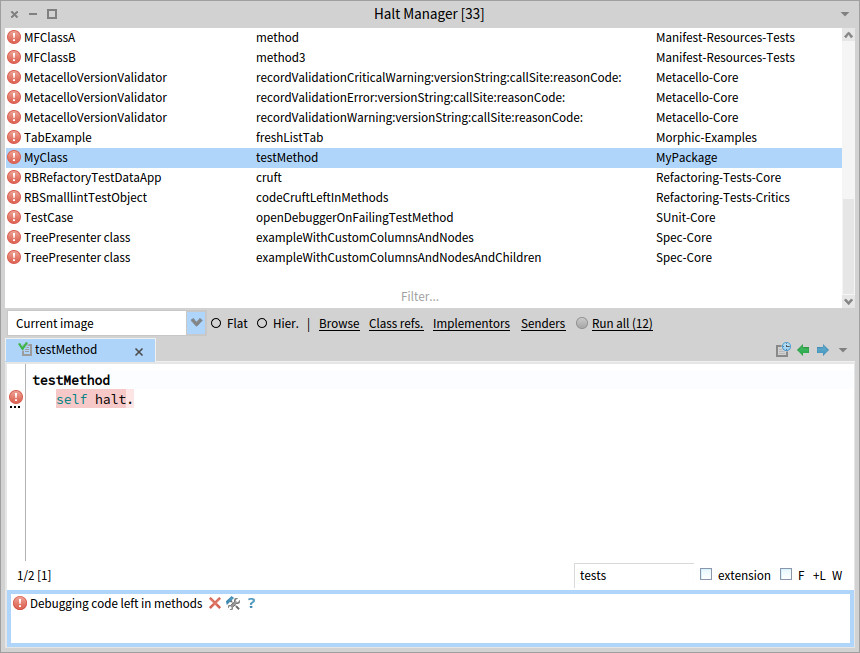
\includegraphics[page=1,width=1\textwidth,frame={\fboxrule}]{./Images/HaltManager.jpg}
   \end{tabular}
 \caption{HaltManager. At the top is a list of all the methods containing breakpoints and halts. At the bottom is the code of the selected method. Hovering over the red orb in the margin will offer the option to toggle the halt message off}
 %\label{fig:Test}
\end{figure}


\paragraph{Improvement of the conditional breakpoints of Pharo.}
In collaboration with Marcus Denker, we improved the conditional breakpoints of Pharo to have the condition expression be executed "as if" it was in the context where the breakpoint was placed, despite this not actually being the case. For this we forwarded the intended execution context to the execution place of the condition and manipulated its abstract syntax tree (AST) to turn variable reads into context lookups of the intended execution context.


\paragraph{AST interpreter.}
I implemented an AST interpreter in Pharo, taking as input the AST of a program and simulating its execution. The goal was to get some experience with how an execution proceeds, as well as being able to control it to prototype debugging tools able to manipulate it in more convenient ways for developers.

% Implementation of an AST interpreter taking as input the AST of some Pharo code and simulating its execution. Originally intended as just an exercise, it was later envisioned to use it as a practice field to develop debugging tools able to manipulate executionsin more convenient ways for the developer.
% Look at the code. Maybe talk about the structure into context.
% Non-local returns
% Problems raised by guille about its lack of support and incorrectness towards some aspec of normal pharo execution (look at worklog). Solving them would require making significant changes to its core structure
% Left on the side for now. Could maybe be redone/extended later or experiments being made with another AST interpreter that looks more comprehensive.

\paragraph{Publication.}
I published thoughts and prototypes for new debugging tools as a position paper named \emph{Analysis and exploration for new generation debuggers}\footnote{https://doi.org/10.1145/3139903.3139910} in the IWS workshop of ESUG 2017.

\paragraph{Expression evaluation recorder.}
This tool is a prototype built with the goal of allowing the developer to access the past state of an execution. It allows to instrument a method by reflectively modifying its bytecode so that whenever one of its expressions is evaluated, the result is copied in a dictionary that can later be accessed by the developer.

\paragraph{Invariant checker.}
Based on the idea expressed by Arya et all~\cite{Arya17a}, this tool is a prototype taking as input an expression (for example returning whether a particular invariant is satisfied) and some code. It first executes the expression, stores its value, then run the provided code while re-executing the expression after each step. If the expression evaluates to a different value than the initial one, the execution is stopped and a debugger opened on the statement that caused this value change. While having limitations, it allows a developer to simply enter an invariant and be shown the point of the program it stops being true.

\paragraph{Debugging of concurrent programs (in progress).}
As part of an ongoing internship at the Soft team of the Vrije Universiteit Brussel, I am collaborating with 1) a project to design a formal semantic for a debugger of concurrent programs that can guide the implementation of an actual debugger and be repurposed for different concurrency models and 2) a remote debugger for big data clusters.


% Partie scientifique

% Partie technique

% Année de recherche au sein de l'Inria et l'université libre de Bruxelles (VUB)
% 	- HaltManager
% 	- Conditional Breakpoint Improvement with marcus
% 	- Interprète d'AST pour maitriser l'exécution et pouvoir prototyper des outils de debuggage dessus

% \begin{itemize}
% 	\item Stage M2 Rmod
% 		\item papier IWST
% 		\item Expression Evaluation Recorder
% 		\item Invariant Checker
% 	\item Année de recherche
% \end{itemize}

% VUB
% 	- travail sur le debuggage de programmes concurrents




\section{D\'emarche}
% Cycle agile. Selectionner ce qui a été fait ou pas. Contruire un prototype pour tester sur un cas un peu plus réel.

The three main intended axis for this thesis are:
\begin{itemize}
\item Back in time debugger
\item Execution Comparison
\item Debugging Specific Language
\end{itemize}

Each of these axis represents a promising, but challenging to precisely define and implement, debugging feature. However, the objective is not simply to develop new debugging feature in a vacuum, it is to develop them so that they can and are used for real by developers. For this reason, the intended workflow is made of agile cycles:
\begin{enumerate}
\item Review of the existing literature on the feature
\item Prototyping the feature
\item Industrial validation of the prototype
\item Adjustments based on the feedback
\end{enumerate}
% \cite{Pers17a}

% Cycle de travail:
% - étude biblio
% - prototypage
% - validation industrielle
% - retour d'expérience

Its powerful reflective abilities and IDE integration, as well as my previous experience with it makes Pharo the programming language/platform of choice to develop the prototypes of this thesis.

\subsection{Back in time debugger}
% Back-in-time debugging.
% Cause du bug n'est plus sur la pile.
% D'ou vient cette valeur?
% Changement d'état est irréversible, donc si on va trop loin dans la simulation de l'éxecution il faut recommencer.

% Prototype de back-in-time debugger
% Possibilité de le scoper pour s'intéresser à certains objets particuliers
A back in time debugger is a debugger that can go backward in an execution. This is especially useful to answer questions like \emph{where does this value come from?} or to find the cause of a bug when it is no longer on the execution stack. Implementing a back-in-time debugger is made challenging by the intrinsic forward nature of executions (variables get overwritten, method calls that return are forgotten, unused memory gets reclaimed...). The two main axis to implement a back in time debugger are 1) storing the state of the execution to go back to it later and 2) re-running the program up until the desired point. These axis show the trade-off between memory usage and time taken to re-execute as a central consideration for the design of a back in time debugger. Beside this consideration are a few key challenges like limiting the runtime overhead, having an acceptable memory use, defining the scope of what should be accessible (whole system?, some objects defined in advance by the developer?) and handling interactions with the outside world (network requests, OS calls...) happening during the execution.

\subsection{Execution Comparison}
% Comment est-ce-qu'on aide le developeur a trouver des régression? Comparer deux piles. C'est mieux à priori de comparer les executions vivantes via debugger que les traces mortes.

% Dans le contexte de la comparaison d'exécution
% étendre les outils existant pour visualiser les executions/piles
The main use-case for this feature is a developer having a version of an application passing some test, modifying its code or giving a different input and having the resulting application fail the test. This feature would allow the developer to debug both executions concurrently, with adapted debugging operations like \emph{Step to the next difference}, to get a better understanding of what makes the second execution fail the test, and the impact his change had. The main challenges for this feature are: what is a definition of \emph{difference} between two executions that would be useful for debugging, and how to recognise matching objects between the two executions (by their state? by how they have been used in the executions?).

\subsection{Debugging Specific Language}
% 1er prototype d'un langage de script pour naviguer ces executions/piles (DBSL)
% 	- step
% 	- boucles... (power of general programming languages)
% 	- définition de conditions sur des patterns
Mainstream debuggers offer basic step commands like \emph{step over} or \emph{step into} as buttons. The idea behind this feature is to give the developer the ability to control the debugger via a Domain Specific Language. For example, this will allow the developer to craft his own step commands like \emph{step into until reaching an object of class C} or \emph{step over until variable V has value W}, to adapt to the particular application that is debugged. A console would be integrated into the user interface of the debugger to give the developer instant access to this potential. Additionally, the debugger could record the step operations performed by the developer so that they can be shared with others to reach a particular point in an execution. The challenges for this feature are: how to design a language that is convenient to use for developers and make their lives easier, what are the basic stepping operations needed so that this DSL can get re-used for other debuggers, how to integrate it with the other two axis of this thesis to allow to script the step back in time and the debugging of two similar execution


\section{Actions pr\'evues pour la premi\`ere ann\'ee}

Work on the Execution Comparison axis: Finding how to compare two living execution stacks and extending existing tools to visualise executions side-by-side. More details in the Execution Comparison part of the D\'emarche section.
Work on the Debugging Specific Language axis: prototyping the scripting language with notably 1) access to the basic step operations of debuggers 2) inclusion of the power of general programming languages (loops, if-then-else constructs...) 3) inclusion of a mean to easily define patterns on the execution stack or the states of objects, to be used as stopping conditions, or patterns to step over for example. More details in the Debugging Specific Language part of the D\'emarche section.


\section{Actions pr\'evues pour la deuxi\`eme ann\'ee}

Work on the Back-in-time Debugger axis: more details in the Back-in-time Debugger part of the D\'emarche section. 


\newpage
\newpage





\subsection{Back in time debugger.}
% Can we implement a back-in-time debugger?

The bug in Pillar is difficult to debug because the stack trace does not contain all the information relevant to the bug.
Indeed, even if we know that the bug's symptom is that the expression \ct{anInput configuration outputType} evaluates to \ct{nil}, we do not know how that value arrived there nor why.

The general problem is that a stack trace shows only a single path in the program's execution.
That is, if we think a program's execution as a call graph~\cite{Grov97a}, the stack trace shown in the debugger represents a single path from that call graph.
In this terminology, a stack trace only shows the current execution path from the program entry point until the break point.
Previous execution paths and their execution contexts are discarded and the state they held is not available for debugging anymore.

This problem also happens with the program state.
A stack trace only provides access to temporary variables in the stack.
Moreover, these values are stored as object references, so if the related objects were modified during in the execution, then the stack trace shows only their last version.
Thus, when using a traditional stack trace, we only have a view at the moment the execution was suspended, and not as they were when these execution contexts were captured.

In order to have access to more information about the execution, without having to constantly place new breakpoints and re-running it, we could store more information as the execution progresses.

Even more information about the execution could be stored by using techniques from the \emph{back-in-time debugging} field \cite{Lewi03a} \cite{Poth07a}\cite{Hofe06b} \cite{Fier09a} \cite{Lien08b}.

\paragraph{Challenges 1: Temporality of the Stored Objects.} A standard issue with storing objects during an execution is their "temporality", as side effects in the following execution may alter them, hence defeating the point of storing them for later review. A simple solution would be to copy the objects and storing the copies instead of the originals, however, this ties into a second challenge.

\paragraph{Challenge 2: Memory Consumption.} A limitation of any storing solution is the memory limit. The evolution of the program state and execution path throughout an entire execution represents a lot of data. To circumvent this limitation, one can restrict the scope of the information stored (for example only storing the evolution of the state of a few objects). Another solution consists in taking advantage of the deterministic nature of executions and only storing some of the states of the execution. Then any state of the execution can be reached by simulating the execution starting from one of these stored states \cite{Arya17a}.  
These two solutions highlight two dimensions of execution information storage techniques: the \emph{granularity} of the storage \ie how much of the execution state do we store, and the \emph{frequency} of the storage \ie at which intervals do we store the state of the execution.


\subsection{Execution Comparison.}
% What would be a language to script the parallel progression of two executions?
% Master-slave execution?
In our Pillar scenario, the developer has two versions of the program: a first one that passes the test and another one that does not. Moreover, he knows what code-change made the test fail. This scenario is similar to the one studied by Zeller et al. in delta-debugging~\cite{Zell05a}.

The developer can then try to compare the execution of the broken program with some other running version of it.
For example, he could try to compare the broken test with its previous version that was working.
Alternatively, he could try to compare the broken test with a working test from the same version of the code.
If the working test exercises the same program but with a different input, it could give her enough insight on the origin of the problem.

In both scenarios, the developer would like the debugger to provide her with information about how the two test executions differ so that he can understand how his change made the test fail. For the sake of presentation, we will focus in the following subsections on the first scenario.

The developer would like to spot differences between the execution paths of the programs.
%A first kind of differences between two executions we would like to spot are the differences between their paths in their control flow graphs.
% A first approach to spot execution differences is to compare their paths in their control flow graphs.
A naive idea to achieve this would be to run the two executions in parallel, compare the sequences of messages sent and stop the executions when they diverge.
This would effectively pinpoint the first path difference between the two executions.
% A tool that would run the two executions in parallel, compare the sequences of messages sent and stop the executions when these sequences diverge would effectively pinpoint the first path difference between the two executions.

Unfortunately, this is most likely not enough to entirely cover the needs of the developer.
For example, the cause of the bug may not be related to the first found difference, but to a difference occurring later in the execution.
% Thus, we need the support to navigate to and from ulterior differences in the execution path.
A possible way to address this concern would be to offer the developer a way to \emph{smart step} from difference to difference, which would step both executions until the next difference.

\paragraph{Challenge: Defining Execution Path Differences.}
Notice we referred to the concept of \emph{differences} between execution paths without precisely defining it.
Indeed, this is to us an open research question: What is a definition of difference that is useful for debugging?
Indeed, a too strict definition of difference (\eg comparing the two sequences of messages and flagging the positions where different messages were sent) would drown the developer in differences instead of showing a bigger picture, delivering a bad debugging experience.
On the other hand, a too relaxed definition of difference could miss some genuine differences.

% Navigating a pair of stacks requires, as we said above, to find differences in the stack.
% We acknowledge this point as an open research question: What would be a good definition of difference?
% Indeed, we believe that a strict definition of difference would spot lots of false positive differences in the stack, forcing the developer to interrupt her debugging process more often and thus, provoking a bad debugging experience.
% On the other hand, a more relaxed difference strategy would cause lots of false negatives, ignoring potential causes of bugs.

Besides a definition of execution path difference, we also need a definition of similarity. As the execution paths advance and diverge, they may converge later if the two executions are similar enough, allowing us to find the next divergence. This problem is particularly challenging when debugging complex applications using big libraries or frameworks because they may have complex execution flows. 

\paragraph{Challenge: Object Equivalence.}


\gp{I propose an alternative version of this paragraph that does not talk about isolation, since we never talked about it before}
Comparing object interactions in both executions requires defining an \emph{object equivalence} criteria. 
Depending on the debugging scenario, we estimate different criterion could be applied.
For example, using strict equality can be useful in the scenario where we debug two versions of the program with the same input.
On the other hand, a more relaxed equality, \eg a manually selection done by the developer, could be useful in the scenario comparing the same program with different input.

Moreover, we identify other open questions related to this topic.
Can we automatically detect and propose the most suitable object equivalence strategy given a debugging scenario?
Given an object equivalence strategy, can we automatically identify pairs of objects representing conceptually the same instance?

\subsection{Debugging Specific Language.}
What would be a list of instructions to add to the debugger to script it? For example being able to express conditions and run the execution until they are satisfied. What are the requirements for the back-end debugger used (for example implementing step over, step into and step through), to maybe be able to export this model onto other debuggers, like gdb, a python debugger etc...
An idea could be to think about adding a command line to the debugger.
A point to think about is how to express a position in an execution.

DSL for Custom Debugger Steps. Mainstream debuggers, to control executions, offer generic step commands usable in most circumstances. However, developers working on specific applications may want to leverage the specificities of these applications to improve their debugging experience. For example, if an application processes data via a succession of operation (a pipeline), developers debugging it regularly may greatly benefit from their debugger integrating specific step commands stepping from an operation to the next.
In this regard, debuggers could include a DSL allowing developers to script new step commands specific to their applications.

\paragraph{Challenge: Expressiveness.} A common point we glossed over in the previous two paragraphs is how to write the expressions or custom debugger steps.
The objects contained in these expressions need to be reachable from the context in which they are evaluated, so these expressions can be evaluated either in the scope of execution context (for example, having access to temporary variables) or in the global scope (only having access to global variables).
Both solutions have drawbacks.
The first one may create unwanted behaviours if multiple unrelated temporary variables across multiple methods have the same names, and requires a semantic for when the expression is evaluated in a context that for example does not contain temporary variables the expression refers to.
The second one requires making relevant objects accessible from the global scope, which poses a constraint on the source code.

\section{Actions pr\'evues pour la premi\`ere ann\'ee}

Comment est-ce-qu'on aide le developeur a trouver des régression? Comparer deux piles. C'est mieux à priori de comparer les executions vivantes via debugger que les traces mortes.

Dans le contexte de la comparaison d'exécution
étendre les outils existant pour visualiser les executions/piles
1er prototype d'un langage de script pour naviguer ces executions/piles (DBSL)
	- step
	- boucles... (power of general programming languages)
	- définition de conditions sur des patterns

\section{Actions pr\'evues pour la deuxi\`eme ann\'ee}

Back-in-time debugging.
Cause du bug n'est plus sur la pile.
D'ou vient cette valeur?
Changement d'état est irréversible, donc si on va trop loin dans la simulation de l'éxecution il faut recommencer.

Prototype de back-in-time debugger
Possibilité de le scoper pour s'intéresser à certains objets particuliers


% Plan by Steph
% ohlalalal debugger c’est dur :)
% pour x y and w reason

% voici ce que l’on compte faire
% 	- scriptable debugger
% 	- master slave mode
% 	- language pour comparer les traces
% 	- invariant checker 
% 	- back in time. 


% Défis: 
% - comparaison d'exécutions (récursion, data-dependent)
% - pas évident de définir la similarité entre deux éxécutions qui sont techniquements distinctes.
% - Applicable à une grosse application (iceberg)?




\newpage
\newpage



\section{abstract}
Locating and fixing bugs is a well-known time consuming task. 
Advanced approaches such as object-centric or back-in-time debuggers have been proposed in the literature,
still in many scenarios developers are left alone with primitive tools such as manual breakpoints and execution stepping. In this position paper we explore several advanced on-line debugging techniques such as advanced breakpoints and on-line execution comparison, that could help developers solve complex debugging scenarios. We analyse the challenges and underlying mechanisms required by these techniques. We present some early but promising prototypes we built on the Pharo programming language.
We finally identify future research paths by analysing existing research and connecting it to the techniques we presented before.


\section{Introduction}

Identifying and fixing bugs is an important task in software development. It is also well-known that this is a time-consuming activity~\cite{Somm01, Zell05a}. 
Several works have been proposed to help developers with such complicated task.
Automatic validation of conditions~\cite{Lenc99a} and watchpoints~\cite{Arya17a} help developers to spot divergences from the expected program execution.
Back-in-time debuggers offer the possibility to navigate the program execution history with several promising research reults~\cite{Lewi03a,Hofe06b,Poth07a,Lien08b}.
%They raised the question of updating and navigating object state is time~\cite{Pluq09b}~\gp{do not udnerstand this sentence}.
More recently, object-centric debuggers presented advanced stepping mechanisms targeting individual objects~\cite{Ress12a}.
Moldable debuggers~\cite{Chis14b} offer a different perspective to this problem: allowing programmers to adapt a debugger to a given domain or task. 

In this position paper we motivate the need to mature and develop more advanced techniques by showing a complex debugging scenario obtained from a real use case.
We then explore several promising advanced debugging techniques and analyse the key challenges they pose:
\begin{description}
\item[Advanced Breakpoints.] What if a developer had the potential to create new smart breakpoints? What would be such breakpoints? What kind of runtime information should they have access to to be both useful and efficient?
\item[Execution Comparison.] What if a developer could, after modifying his codebase and breaking some tests, compare the executions of the program before the change and after the change to find the cause of the bug? What would be the infrastructure required for this technique? What are the tools we could provide to a developer to perform this task?
% \item[Execution Comparison.] What if a developer could easily debug in parallel the same program with slight variations to compare the behaviour and find the cause of a bug? What is the infrastructure required for that scenario? What are the tools that we could provide to a developer to simplify the comparison of both executions?
\item[Accessing Execution History.] Back-in-time debuggers are nowadays the referent debuggers to navigate history. However, many questions remain still open. What would be a both a practical and efficient solution? What are the alternatives to store both the execution and the objects in the program's state? How can we navigate the program history to find a bug?
\end{description}

During our analysis, we also present some promising ideas like the possibility of scripting the stack navigation.
Finally we present some prototypes we implemented showing the feasibility of some of them. 


% In this section we present some common debugging scenarios that developers face and that are not really well covered by existing toolset. 
% We describe a typical scenario, \gp{you already said in the previous sentence that you'll present scenarios, so the last 5 words are useless} explain what a developer could use to identify the bugs. Such scenarios can be addressed in different manners and an analysis of the underlying 
% mechanisms that are needed to implement advanced debuggers is presented in the subsequent section. \gp{avoid passive voice. We present in the following sections an analysis of...}

\section{A Real Complex Debugging Scenario}\label{secscenario}

To illustrate why debugging is a complex task and motivate the need of new debugging techniques, we isolated a real bug that appeared while refactoring the latest versions of the Pillar markup language\cite{Arlo16a}. In this section we present the issue found and the way to reproduce it. We setup a repository explaining in details the steps to reproduce the bug in \url{https://github.com/guillep/pillar-bug},

Pillar uses an object called \ct{PRPillarConfiguration} to manage all project settings \eg what is the output format, whether it needs to numerate sections or not, print a contents table or not. \ct{PRPillarConfiguration} semantics are complicated. First, it overrides \ct{doesNotUnderstand:}~\cite{Duca99a} to dynamically interpret some message sends as configuration setters or getters. Second, it uses the Magritte~\cite{Reng06a} meta-description framework to control how a configuration values should behave by default, be serialized, deserialized, and validated. Finally, a \ct{PRConfiguration} is organised in a hierarchy of configurations, and some operations may lookup settings in the hierarchy of the configuration while others do not.

Given this situation, the pillar developers decided to refactor \ct{PRPillarConfiguration} to depend less on \ct{doesNotUnderstand:} semantics.
They so decided to introduce in \ct{PRPillarConfiguration} a \ct{disabledPhases} instance variable with its respective accessors.
Before doing such a change, all 3182 Pillar tests were running ok.

\begin{lstlisting}[language=bash]
$ ./pharo Pharo.image test "Pillar.*"
[...]
3182 run, 3182 passes, 0 failures, 0 errors.
\end{lstlisting}

However, as soon as we introduce the new accessors, 16 new errors appeared:

\begin{lstlisting}[language=bash]
$ ./pharo Pharo.image test "Pillar.*"
[...]
3182 run, 3166 passes, 0 failures, 16 errors
\end{lstlisting}

Checking the tests, we observe that the bug happens in an apparently unrelated piece of code, the \\ \ct{PREPubMenuJustHeaderTransformer$>>$actionOn:} method.
The symptom of the bug is that \ct{outputType} is nil. However, this piece of failing code plus the fact that 3166 tests are still working, give us no clue about the relation with the change and the bug.

\begin{lstlisting}
PREPubMenuJustHeaderTransformer>>actionOn: anInput
  ^ (self class writers
    includes: anInput configuration outputType writerName)
    ifTrue: [ maxHeader := self maxHeaderOf: anInput input.
      super actionOn: anInput ]
    ifFalse: [ anInput ]
\end{lstlisting}

In the following sections of this paper, we explore several advanced debugging techniques that could help us finding the cause of this bug.

\section{Technique 1: Advanced Breakpoints}\label{secbreak}
Breakpoints are a very common feature among debuggers.
They let developers specify a point in a program where the execution should be suspended.
However, debuggers usually limit breakpoints to a limited set of pre-existing ones such as breaking when the program arrives to a particular line.
Developers are not usually capable of tailoring breakpoints to some more specific needs.
This section presents some ideas that would increase the expressiveness of breakpoints and allow developers to specify more precise trigger conditions.

\subsection{Idea 1: Conditional Breakpoints}

\paragraph{Scenario.} The developer debugging Pillar is interested in looking at what happens to the problematic \ct{actionOn:} method only when it is called with a specific argument. If he places a normal breakpoint in the method, the breakpoint will trigger no matter the argument and he will have to check himself whether the arguments are those he is interested in.

\paragraph{Idea.} The developer could place a \textit{conditional breakpoint} that only triggers if the arguments are those he is interested in.
Conditional breakpoints are nowadays available in many existing debuggers such as Pharo's and C's gdb, mostly allowing the execution of simple conditional expressions.
We would like to explore their limitations and further possibilities.

% [Pharo offers conditional breakpoints that can stop depending on a caller chain or a specific predicate.] \td{This looks like implementation detail to me}
%\gp{We should extend this a bit more. Most debuggers can do conditional breakpoints. But they are just very primitive. What is the difference between this idea and what already exists in a C debugger or Pharo?}

\subsection{Idea 2: Contextual Breakpoints} 

\paragraph{Scenario.} The Pillar developer would like her breakpoints to only be triggered when her code is launched from a test. A normal breakpoint triggers from any execution, whether a test or not. This may interfere with the normal execution of the program, even in cases where the bug does not reproduce or appear.

\paragraph{Idea.} The developer could place a \textit{contextual breakpoint}: a conditional breakpoint that depends on the dynamic execution of the program. For example, a breakpoint could detect whether the current execution was initiated by a test process or not, or by an HTTP request or not. Moreover, this selective breakpointing could be useful to debug core libraries such as collections or compilers. Since core libraries are in usage by the runtime, setting a breakpoint in the may cause the entire runtime to suspend.

\paragraph{Alternative Scenario.} A developer wrote a test to validate his implementation. He placed breakpoints in different methods invoked in the test because he is adjusting the behaviour of such methods to make the tests pass.
Alternately, he may want that when executing the test, only the breakpoints placed in the test method itself trigger.

% The inverse scenario is also interesting. The developer wrote a test to validate its implementation. He also placed break points inside different methods invoked by the test because he is adjusting the behavior of such methods to make the tests pass. He goes from one break point to another to validate his implementation. He should be able to:
% \begin{itemize}
% \item stop in the breakpoints inside his methods but only when he is not executing the code from the test. This way he can verify and modify the methods. 
% \item when the test is executed only break points inside the test method are active and all the break points in is methods are ignored. 
% \end{itemize}




% [Scenario for the context-specific breakpoint, based on: "\textit{context-specific breakpoints}, for example breakpoints that only stop the execution when being encountered while running a specific test, or while not running any test. This way they can be let at relevant locations of the source code for later use without interfering with other activities."]
% Breakpoints are a very common feature among debuggers. As such, improving their expressiveness, and therefore their ease of use for developers could significantly improve the debugging experience. A few examples include:
% \begin{itemize}
% \item \textit{conditional breakpoints}, breakpoints that only stop the execution of the program if a certain condition specified by the developer when placing the breakpoint is fulfilled.
% \item \textit{context-specific breakpoints}, for example breakpoints that only stop the execution when being encountered while running a specific test, or while not running any test. This way they can be let at relevant locations of the source code for later use without interfering with other activities.
% \end{itemize}

% Uses for breakpoints that work only in tests:
% - Debugging morphic: putting a normal breakpoint in morphic means that the UI will not continue to work
% - Debugging the pharo compiler: after putting a breakpoint in the compiler code, the compiler won't be able to compile this code because it will break.sm


\subsection{Challenges}
These ideas rely on the possibility for the breakpoints to decide whether to trigger based on the context they are executed in.
This means that the breakpoints must be able to access their context, which is not trivial in most languages.
Moreover, we ask ourselves the following research questions:
What is the debugger support required to interactively set conditional breakpoints?
What is the runtime information they can and could access?
How could we easily define dynamic contexts that would help debugging?

% This scenario shows that being able to specify and use an execution context is important to create advanced break points. 
% By default a system can provide a specific context for test execution. Now the question of the possibility by the developer to create
% on the fly such creation context should be investigated. 
% \td{Saying it's hard because it requires access to the process we are in to know if we have been launched by a test?}
\gp{Check this paper: \url{https://scm.gforge.inria.fr/authscm/gpolito/svn/lse/Papers/2014-WISIT-Breakpoints/}}
\sd{guille should we put a ref to this paper?}
\gp{dont know, we send it to a small small small workshop in argentina. It was mostly to support them. But the paper is not online, nor anything...}

\section{Technique 2: Execution Comparison}\label{secspot}
%\subsection{Execution Comparison}
% \td{I think "Execution Comparison" is simpler to grasp. It does not really depends on the solution in my opinion, it's just that the scenario is about a developer that would like to compare two executions to find how they differ.}

\subsection{Scenarios}
In our Pillar scenario, the developer has two versions of the program: a first one that passes the test and another one that does not. Moreover, he knows what code-change made the test fail. This scenario is similar to the one studied by Zeller et al. in delta-debugging~\cite{Zell05a}.

The developer can then try to compare the execution of the broken program with some other running version of it.
For example, he could try to compare the broken test with its previous version that was working.
Alternatively, he could try to compare the broken test with a working test from the same version of the code.
If the working test exercises the same program but with a different input, it could give her enough insight on the origin of the problem.

In both scenarios, the developer would like the debugger to provide her with information about how the two test executions differ so that he can understand how his change made the test fail. For the sake of presentation, we will focus in the following subsections on the first scenario.

% \begin{figure}[!htp]
% \begin{center}
% 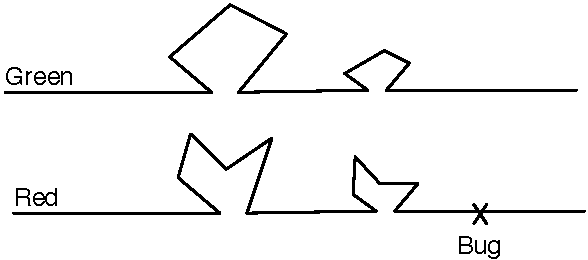
\includegraphics[width=0.9\linewidth]{figures/TwoExecutions.pdf}
% \caption{An execution path not breaking tests and one breaking test.}
% \end{center}
% \end{figure}

% \paragraph{Scenario.} When working on large applications, it is not uncommon to start from a version that passes all the tests and make a change that causes one test to fail, while having no clue what the relation between the change and the test is. In this setting, the developer has two versions of the program: one that passes the test and another that does not.

% \paragraph{Scenario.} When working on large applications, it is not uncommon to start from a version that passes all the tests and make a small change that causes one test to fail, while having no clue what the relation between the change and the test is. In this case, the developer would have to find the point where the execution "goes wrong" to figure out how his change impacted the failing test.

% \paragraph{Wish.}
% The debugger could assist the developer by comparing the execution of the current version where the test is failing to the execution of the previous version where the test was passing, by stepping through both executions in parallel and finding the point where they stop being "similar". This notion of "similar" could be expressed in terms of stack comparisons: two execution are similar if their stacks are equal. This would allow the developer to quickly find where his change made the execution diverge from the correct one of the previous version.
% However, maybe the first divergence between the two executions has nothing to do with the test, for example because the change affected a method that was also used elsewhere than in the system covered by the now failing test. To take this into account, the debugger could offer more general functionalities such as:
% \begin{itemize}
% \item from two dissimilar executions, step through both executions until they become similar again
% \item starting with two dissimilar executions, step through both executions until they become similar again
% \end{itemize}
 

% The debugger could assist the developer by comparing the execution of the current version where the test is failing to the execution of the previous version where the test was passing, by stepping through both execution in parallel and finding the points where they are not "similar". This notion of "similar" could be expressed in terms of stack comparisons: two execution are similar if after the same number of steps, their stacks are equal.


%\td{Code like this:?}
%\begin{lstlisting}[caption=Test]
%testGenerateBookID
% |bookID bookTitle|
% bookTitle := 'Alice in Wonderland'.
% bookID := BookManager generateBookID: bookTitle.
% self assert: bookID equals: '#-', bookTitle.
%\end{lstlisting}
%\begin{lstlisting}[caption=Method in working version]
%generateBookID: aString
% ^ '#-',aString
%\end{lstlisting}
%
%\begin{lstlisting}[caption=Method in failing version]
%generateBookID: aString
% ^ '#_',aString
%\end{lstlisting}
%\sd{I would comment it. I do not really think that this example catch the problem. I have the impression that a picture showing two executions would be better because there are parts that we want to skip. }


%\paragraph{Paired executions.} 



% A basic idea is to have the debugger run the two executions of the test in parallel, stepping through them until they stop being "similar". [The Red path is stepped using the information in the Green Path. ]

% This requires a process being able to remotely control two isolated executions at the same time and examine their stack and memory state, as well as a definition of "similarity". 


% \subsection{Idea 1: Showing and Navigating Execution Path differences}
\subsection{Idea 1: Comparing Execution Paths}

The developer would like to spot differences between the execution paths of the programs.
%A first kind of differences between two executions we would like to spot are the differences between their paths in their control flow graphs.
% A first approach to spot execution differences is to compare their paths in their control flow graphs.
A naive idea to achieve this would be to run the two executions in parallel, compare the sequences of messages sent and stop the executions when they diverge.
This would effectively pinpoint the first path difference between the two executions.
% A tool that would run the two executions in parallel, compare the sequences of messages sent and stop the executions when these sequences diverge would effectively pinpoint the first path difference between the two executions.

Unfortunately, this is most likely not enough to entirely cover the needs of the developer.
For example, the cause of the bug may not be related to the first found difference, but to a difference occurring later in the execution.
% Thus, we need the support to navigate to and from ulterior differences in the execution path.
A possible way to address this concern would be to offer the developer a way to \emph{smart step} from difference to difference, which would step both executions until the next difference.




% We should be able to compare two different execution paths by just comparing message sends. This approach focuses on the path in the control flow graph the two executions are following. A tool that would run the two executions in parallel, compare the sequences of messages sent and stop the executions when these sequences diverge would effectively pinpoint the first path difference between the two executions.

%Unfortunately, this is most likely not enough to entirely cover the needs of the developer. For example, if he changed a method that is used multiple times in the execution of the test, but only the, say third, call to it causes the test to fail, then this tool would not help him at all.


% The developer could then access the third point where the method he changed by using this stepping mechanism just a couple of times.

% Something to note is that the developer may want to automate this process of reaching the third path difference between the execution for rapid testing iterations. A Domain Specific Language (DSL) could help him to script the debugger to automatically pilot the two executions.

% A first approach is to compare message names.  This first idea is also incomplete, as it could happen that the developer changed a method that is used multiple times in the test's execution, but only the, say third, call to it causes the test to fail. The debugger feature of finding the first divergent point would point the developer at the first time this method is called (because since it is different, it causes the stack or the state to differ) and not the third call where the problem actually occurs. At this point, if the change in the method made it one step longer or shorter, then the two executions will never be similar again, as they will be "desynchronised", preventing the same technique from being used to reach the second or third call of the method.

% Other features like allowing the developer to specify a list of messages the debugger should not consider different even if they are, stepping through both executions until a given message is sent a given number of times could also be evaluated. \gp{a bit redundant with the challenges, no? also, we should avoid passive voice. Better start with "We evaluate also..."}

% What this analysis stresses is that it is important to be able to specify that a given execution path is not interesting and should not consider it during the stack match. The way to express such situation should be investigated. We foresee several approaches: the developer may want to say "try to arrive the same messages", the same occurrence of messages (meaning arriving to the third time a given message is sent), or express it negatively by specifying to skip a specific call, or all the messages of a certain kinds.

\paragraph{Challenge: Defining Execution Path Differences.}
Notice we referred to the concept of \emph{differences} between execution paths without precisely defining it.
Indeed, this is to us an open research question: What is a definition of difference that is useful for debugging?
Indeed, a too strict definition of difference (\eg comparing the two sequences of messages and flagging the positions where different messages were sent) would drown the developer in differences instead of showing a bigger picture, delivering a bad debugging experience.
On the other hand, a too relaxed definition of difference could miss some genuine differences.

% Navigating a pair of stacks requires, as we said above, to find differences in the stack.
% We acknowledge this point as an open research question: What would be a good definition of difference?
% Indeed, we believe that a strict definition of difference would spot lots of false positive differences in the stack, forcing the developer to interrupt her debugging process more often and thus, provoking a bad debugging experience.
% On the other hand, a more relaxed difference strategy would cause lots of false negatives, ignoring potential causes of bugs.

Besides a definition of execution path difference, we also need a definition of similarity. As the execution paths advance and diverge, they may converge later if the two executions are similar enough, allowing us to find the next divergence. This problem is particularly challenging when debugging complex applications using big libraries or frameworks because they may have complex execution flows. 

% Moreover, a definition of execution path difference must also include a definition of similarity. As the stacks advance and diverge, we expect that they will also converge later on, to naturally continue a debugging session. This problem is particularly challenging when debugging complex applications using big libraries or frameworks because they may have complex execution flows. 

% \subsection{Idea 2: Showing and Navigating Object State Differences}
\subsection{Idea 2: Comparing Object Interaction History}

The developer would also like to spot differences between the interactions with some particular object(s) in both executions.
%Another kind of differences we would like to spot are the differences between the interaction histories of the two versions (one in each execution) of some objects.
For example, we would like to compare the times an object was sent a particular message in both executions.
Moreover, this idea can also be applied to track the evolutions of the state of an object.%, or to spot the the point in the executions where both versions of the object received a given message for the $n$-th time. 
%For example, we would like to see the differences between the evolutions of the state of an object in both executions, or get to the point in the executions where both versions of the object received a given message for the $n$-th time. 
Similarly to the Execution Path Differences idea, we could offer the developer a \emph{smart step} that would allow him to navigate the executions according to what happens to a given object.

% A first kind of differences between two executions we would like to spot are the differences between their paths in their control flow graphs.

% A second approach to address this debug scenario is to compare the state of the objects instead of the execution stack. Let's consider that a developer may want to compare how a given object's state diverges between the two pair of executions. Or when it is changed or accessed for the nth time. In such case the developer is more interested in the difference between objects than the difference in the stack. A developer can then benefit from a \emph{smart step} that takes into account object differences instead of execution differences.


% Something to note is that the developer may want to automate this process of reaching the third path difference between the execution for rapid testing iterations. A Domain Specific Language (DSL) could help him to script the debugger to automatically pilot the two executions.

\paragraph{Challenge: Object Equivalence.}


\gp{I propose an alternative version of this paragraph that does not talk about isolation, since we never talked about it before}
Comparing object interactions in both executions requires defining an \emph{object equivalence} criteria. 
Depending on the debugging scenario, we estimate different criterion could be applied.
For example, using strict equality can be useful in the scenario where we debug two versions of the program with the same input.
On the other hand, a more relaxed equality, \eg a manually selection done by the developer, could be useful in the scenario comparing the same program with different input.

Moreover, we identify other open questions related to this topic.
Can we automatically detect and propose the most suitable object equivalence strategy given a debugging scenario?
Given an object equivalence strategy, can we automatically identify pairs of objects representing conceptually the same instance?
%We referred to the "two versions" of an object. However, since the two executions are isolated, they do not share objects. Identifying pairs of objects that "represent the same object" in both executions is an open research question.

% Isolating the debugged executions means also that objects are not shared between these processes.
% This poses a challenge to be able to navigate and identify object differences between both stacks.
% Indeed, to track object differences we need to first manage object identify and object equivalence between the two debugged processes. 
% An internal identification mechanism may be a solution \gp{how?}.

\subsection{Technical Challenge}

\paragraph{Running and Isolating two Simultaneous Executions.}
\gp{I propose to remove this section, it is small and finally it does not add too much from a research point of view. what do you think?}
Both of the ideas we expressed in this section relies on the ability of the debugger to run and control two executions at the same time in an isolated fashion.
The isolation is important to prevent the two processes from interfering with each other, for example by accessing the same global variable

%\subsection{Idea 1: Controlling two parallel executions}
% A basic idea is to have the debugger run and control the two executions of the tests in parallel. This requires a process being able to control and isolate two executions, and examine their stack and memory state.

% A technical challenge that needs to be tacked before being able to explore these ideas is to be able to run and control two executions at the same time in an isolated fashion.
% This is important to avoid the debugged processes interfering with each other.
% This would be for example the case of a pair of programs using and updating the same global variable.


% \begin{figure}[ht]
% \begin{center}
% 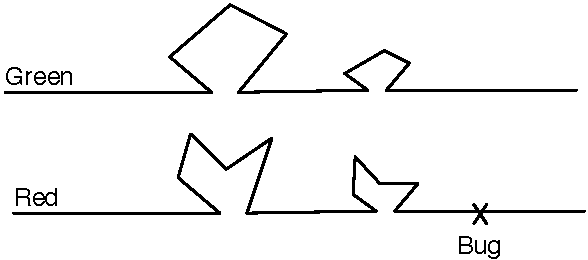
\includegraphics[width=0.9\linewidth]{figures/TwoExecutions.pdf}
% \caption{An execution path not breaking tests and one breaking test.\label{fig:divergence}}
% \end{center}
% \end{figure}

% \paragraph{Isolating Program Executions and Object Equivalence}

% What the scenario (Different Input - Same Code) illustrates is that we need to offer a way 
% \begin{itemize}
% \item to track object use and object state modification, 
% \item then to control the stack stepping based on object use and object changes,
% \item to compare the execution of the Red and Green execution based on such information. 
% \end{itemize}

% The developer may want to go to the point in the Red Stack where a particular object has been changed for the second times. 
% Then he may want to compare the path to arrive to this state, 
% \sd{I believe that one day we will publish a real paper on this and we will set the vocabulary: path = sequence of message, stack synchronise}

% \paragraph{Detecting Execution Divergences and Convergences}

% Another question is how the state in one stack can be used to drive the stepping of the other one. Since objects in each stack will not be shared, an internal identification mechanism may be a solution. The developer may want to say when the third receiver object receive or is passed as argument then stop the stepping. 

% What this scenario highlights is that we should investigate several ways to pattern match the stack structure and state taking potentially into account a second stack.

% \paragraph{Found a good definition of similarity}
% A natural definition for the "similarity" is the following:
% \begin{defn}Two executions are "similar" up to a given number of steps $n$ if their stacks and memory states at any step $n'$ (with $n' < n$) are the same.\end{defn}

%  A challenge with this definition is to establish that two stacks (or program states) are "the same" while they originate from different executions and therefore do not share memory pointers or object identity. 

% \gp{Question/idea: Could we have a smarter step "step until next divergence"?}
% \sd{I think that we should have that and play with it. }
% \td{The last sentence of this paragraph is about why it wouldn't work, because the exexcutions will stay asynchronous forever... Or maybe I misunderstood you?}\sd{Guille we can have one but we also want more because may be you want to skip over the call tree and ignore it.}

% \subsection{A First Conclusion}
% As a first step to address this problem, a debugger should be able to manipulate two stacks and that one of the stack becomes a master or slave to the other stack. Then such debugger should offer step until next divergence functionality.

% Another important point to stress in this scenario is to see that a same object (same identity) in one stack may have different states at different moment. From an implementation point of view, this raises the question of how to support back in time behavior \cite{Lien08b,Pluq09b}.


\section{Technique 3: Accessing Execution History}

\subsection{Scenario}

The bug in Pillar is difficult to debug because the stack trace does not contain all the information relevant to the bug.
Indeed, even if we know that the bug's symptom is that the expression \ct{anInput configuration outputType} evaluates to \ct{nil}, we do not know how that value arrived there nor why.

The general problem is that a stack trace shows only a single path in the program's execution.
That is, if we think a program's execution as a call graph~\cite{Grov97a}, the stack trace shown in the debugger represents a single path from that call graph.
In this terminology, a stack trace only shows the current execution path from the program entry point until the break point.
Previous execution paths and their execution contexts are discarded and the state they held is not available for debugging anymore.

This problem also happens with the program state.
A stack trace only provides access to temporary variables in the stack.
Moreover, these values are stored as object references, so if the related objects were modified during in the execution, then the stack trace shows only their last version.
Thus, when using a traditional stack trace, we only have a view at the moment the execution was suspended, and not as they were when these execution contexts were captured.

%\begin{figure}
%\begin{lstlisting}
%main
%  |intBox|
%  intBox := IntBox new: 1.
%  intBox set: 2.
%  self halt.
%\end{lstlisting}
%\caption{Test}
%\end{figure}
%
%\td{figure showing the execution context tree of the execution of this snippet, and also showing the information missing from the stack trace obtained from the self halt}

\subsection{Idea 1: Storing the History of Executions}

% \subsection{Idea 1: Storing the History of Executions}

% First way: re-executing (naive).

% Second way: store.

% Challenges:
% - Resource (time, memory) consumption
% - Frequency and granularity of the storage

% The simple and naive method to get more information about the execution is to place a breakpoint at the point of interest and re-run the execution. This gives access to the entire state of the program at this point. And by the somewhat tedious process of placing enough breakpoints and manually stepping through the execution, a developer can observe the path of the execution and of the evolution of the state of some objects.
% This method can be summarised as \emph{re-running the execution} to access more information.

In order to have access to more information about the execution, without having to constantly place new breakpoints and re-running it, we could store more information as the execution progresses.

\paragraph{Storing the Result of Expressions Evaluations.} A first way the debugger could provide more information to developers is to store the results of the evaluation of the expressions (and their sub-expressions) in the execution as it progresses. These results could then be displayed to developers to improve the debugging session.

\paragraph{Storing the Entire Execution History.} Even more information about the execution could be stored by using techniques from the \emph{back-in-time debugging} field \cite{Lewi03a} \cite{Poth07a}\cite{Hofe06b} \cite{Fier09a} \cite{Lien08b}.

\paragraph{Challenges 1: Temporality of the Stored Objects.} A standard issue with storing objects during an execution is their "temporality", as side effects in the following execution may alter them, hence defeating the point of storing them for later review. A simple solution would be to copy the objects and storing the copies instead of the originals, however, this ties into a second challenge.

\paragraph{Challenge 2: Memory Consumption.} A limitation of any storing solution is the memory limit. The evolution of the program state and execution path throughout an entire execution represents a lot of data. To circumvent this limitation, one can restrict the scope of the information stored (for example only storing the evolution of the state of a few objects). Another solution consists in taking advantage of the deterministic nature of executions and only storing some of the states of the execution. Then any state of the execution can be reached by simulating the execution starting from one of these stored states \cite{Arya17a}.  
These two solutions highlight two dimensions of execution information storage techniques: the \emph{granularity} of the storage \ie how much of the execution state do we store, and the \emph{frequency} of the storage \ie at which intervals do we store the state of the execution.

\subsection{Idea 2: Navigating the History of Executions}
Another important aspect of helping developers to debug by showing them more information is providing them with tools allowing them to quickly find the information they need.

\paragraph{Expression Watchpoint.} Sometimes developers know the cause of a bug (for example a collection containing corrupted values is sent as argument to a function, that cannot process it and raises an exception) but cannot locate the the point in the execution where this cause appeared (in this example, when did the collection become corrupted). To solve this issue, they could write an expression that would evaluate to true as long as the execution is in a non-bugged state (in this example, the expression would return whether the collection is not corrupted) and have the debugger run the execution and suspend it when the expression evaluates to a different value.

\paragraph{DSL for Custom Debugger Steps.} Mainstream debuggers, to control executions, offer generic step commands usable in most circumstances. However, developers working on specific applications may want to leverage the specificities of these applications to improve their debugging experience. For example, if an application processes data via a succession of operation (a pipeline), developers debugging it regularly may greatly benefit from their debugger integrating specific step commands stepping from an operation to the next.
In this regard, debuggers could include a DSL allowing developers to script new step commands specific to their applications.

\paragraph{Challenge: Expressiveness.} A common point we glossed over in the previous two paragraphs is how to write the expressions or custom debugger steps.
The objects contained in these expressions need to be reachable from the context in which they are evaluated, so these expressions can be evaluated either in the scope of execution context (for example, having access to temporary variables) or in the global scope (only having access to global variables).
Both solutions have drawbacks.
The first one may create unwanted behaviours if multiple unrelated temporary variables across multiple methods have the same names, and requires a semantic for when the expression is evaluated in a context that for example does not contain temporary variables the expression refers to.
The second one requires making relevant objects accessible from the global scope, which poses a constraint on the source code.





% DSL for debugger stepping.

% Writing an expression and reach the point in the execution where it goes from false to true (or some other values at the developer's choice).

% Challenges:
% - Exprimer -> reachability
% - Comment on exprime
% - Qu'est ce qu'on exprime

% \gp{This looks like terminology...}
% One of the main debugging resources for a developer is the stack trace.
% The stack trace is a sequence of executions context that represents the execution path from what we usually call a \emph{program entry point} to the execution context where the execution was suspended by either a breakpoint or an exception.
% This entry point is in most programming languages the \ct{main} function.
% In Pharo, a program entry point is the first context of a \ct{Process}, usually executing the \ct{Block$>>$\#newProcess} method.

% The utility of the stack trace is twofold. 
% On the one hand, it can be used to navigate the execution path and control flow that led to a problem.
% On the other hand, it can also be used to inspect the state of the execution at the moment a bug appeared. This state is composed both by the program global state and the state held by the stack trace \ie object references held in temporary variables.

% \gp{Maybe we need to add a picture of the call graph to explain better}
% Traditional debuggers only allow developers to navigate and inspect the stack trace at the moment where the bug appeared, providing a single path in the program's execution. That is, if we think a program's execution as a call graph~\cite{Grov97a} the stack trace shown in the debugger represents a single path from that call graph.
% This means that previous execution paths from that call graph are lost.
% Execution contexts that already returned were discarded and the state they held is not available for debugging anymore.

% \gp{make a paragraph about why this makes debugging difficult}
% Moreover the current state of the program is the result of a series of side effects  have been subject of several side effects during the program execution.

% \gp{review this paragrpah}
% A developer observes a bug and would like to find the error in the code that generated this bug. The observed bug and the code error may be very far away from each other, and the developer has no clue where the error could be located, so placing breakpoints and stepping through the execution may take a long time. What the developer would like is a way to quickly locate the error in the code that generated the bug he observed. [We need a good solution to navigate history.]
% What the developer would like is a way to find where 

% \paragraph{Objectives.} In this section, our objective is twofold. First, we want to remember more from the execution than the information available in stack traces. Then we want to provide convenient ways for developers to access what they are interested in among these information.

% \td{I don't know what happened to the rest of this section. The part about back-in time is gone, which I guess was because it was an idea from another paper, but then why is the idea about transition watchpoint still here? }

% \subsection{Idea 1: Rebuilding the past state of the execution}
% A naive method to achieve this would be to redo the execution and evaluate the expression written by the developer after each step. The main limitation with this solution is the tremendous time overhead generated if the expression is computationally complex (an example of expression could be to check that a given tree is indeed a tree and does not contain cycles).

% For computationally complex expressions, another method could be used: taking snapshots of the memory and call stack at some points during the execution, assuming the expressions evaluates to true at the start, and to false at the end (where the bug is observed) and performing a binary search over these snapshots to find the closest snapshots surrounding the/a (there may be multiple) point in the execution where the expression evaluates to false.

% Then, the naive method could be applied from the oldest (with regards to the execution) bounding snapshot to find the exact step where the expression evaluates to false.

% One of the challenges would be to be able to access the different snapshots and evaluates the expression set by the developer in their context. Since the snapshots are images of the past, sockets and pipe that were used at that time may no longer be open when evaluating the developer's expression.
% \gp{This is a problem of this section and 2.2. Actually, if you want to replay execution, you need to take care about everything that has a side effect. This should be clear in the paper.}

% \subsection{Idea 2: Storing Intermediate Results}\label{secsinter}

% A developer may want to access the value of the previously executed expressions~(and their sub-expressions). A first manual approach would be for the developer to introduce a temporary variable for each expression he is interested in, to hold its result.
% If it appears that the chosen expressions are not related to the bug the developer should insert a new temporary variable for another expression.
% This leads to a tedious trial-and-error debugging process.
% Moreover, this forces the developer to muddy the code-base with debugging code that then needs to be manually removed later on. 

% A more advanced approach would be to... \gp{explain here the intermediate expression solution}
% a temporary variables holding the result of each expression, and this especially for expressions already executed. With current debuggers, it is tedious to open such results, the developer should anticipate his wish and put a break point before the expression he wants to study and then perform a step over while making sure that he will get the results of the expression. The Pharo debugger offer the topStack variable pointing to the last executed expression to somehow cover such need. 
% The debugger could make the experience of stepping through an execution more informative by showing this additional information to the developer.

% The issue with this approach is the "temporality" of the results. Imagine that the break point stops the execution at the end of a sequence of expressions. If an expression returns an object ($o \rightarrow v1$) and then the following expressions modify this object state ($o \rightarrow v2$). When the developer looks at the first expression value, he sees the object as it is at the end of the expression execution ($v2$) while he should get ($v1$). This problem is related to the issue of versioning and navigating the history of a graph of objects as in Back in time debuggers \cite{Pluq09b}.

% To solve this issue, one could make a copy of the result before storing them, so that they are unaffected by further expression evaluation. However, this also requires copying all the objects this result points to, for the same reason. And this would have to be done for every expression and sub-expression encountered during the execution, leading to a very large memory footprint.

% Two approaches come to mind to solve or diminish this memory problem:
% \begin{itemize}
%   \item Restricting the areas of the source code where this memorisation process happens. For example by explicitly asking the developer to mark the methods he wants to be instrumented.
%   \item Using techniques from the back-in-time debuggers, that are facing the same memory footprint issues \cite{Lien08b}.
% \end{itemize}

% % \paragraph{Analysis.} 
% % The naive idea to implement this feature is to use code rewriting techniques to store the results of the evaluation of the expressions as the program is executed. This information is then displayed by the debugger when the execution is interrupted.

% % The naive idea to implement this feature would be to use reflectivity to alter every ast nodes so that they  \gp{Reflectivity is an implementation detail. Maybe you can say that we will use code rewriting to capture all intermediate states in the execution of a method and show it afterwards?}, after being evaluated during the execution, store the result of this evaluation for further use by the debugger. 

% % \paragraph{Analysis.} The most immediate challenge with this feature is the potentially massive volume of data generated by storing the results of the evaluations of all expressions (and their sub-expressions). But besides this challenge lies a more subtle one: the "temporality" of the results. For example, if an expression would return an object, then the evaluation of the following expressions could modify the state of this object and when the developer would take a look at the results of the first expression, he would see the object as it is now: after the following expressions were evaluated, but not as it was when the execution had not gone further that this expression.

% %A developer observes a bug and would like to find the error in the code that generated this bug. The observed bug and the code error may be very far away from each other, and the developer has no clue where the error could be located, so placing breakpoints and stepping through the execution may take a long time. What the developer would like is a way to quickly locate the error in the code that generated the bug he observed.

% % [Earlier paragraph by stephane:
% % Often a bug is revealed up in one version and it has to be traced back to its introduction. The problem is that a large period of time may have been elapsed between the bug introduction and its notice. A typical debug scenario is to be able to recreate the situation and to identify the problem. Dicotomic searchs and delta debugging offers solutions. What is also challenging is how to identify a bug and the conditions that led to it.]

% %[We need a good solution to navigate history.]

% %\textit{Transition watchpoints} \cite{Arya17a} achieve this by allowing developers to write an expression that evaluates to false (or another specific value) at the point in the execution when the error happens. Typically, the developer would write an invariant he assumes the execution satisfies, but the presence of the bug shows it is violated at some point during the execution.

% \subsection{Challenges}

% \paragraph{Navigating the history.}
% In addition, another challenge is the expressiveness of the developer's expression. Since this expression has to be executed in an arbitrary context (because it can be executed at any time in the execution), it would not make much sense to allow references to, for example, variables that are local to some methods. A simple solution would be to only allow references to global variables, that are always available at any point in the execution, but this puts constraints on the source code, as the variables the developer's expression needs were probably not exposed with such a large scope. A query language for the state of an execution (stack plus memory) could be a way to increase the expressiveness of the developer's expression, allowing to access, for example, all objects of a certain class and check that they are all initialised.

% \gp{I feel this section mixes a couple of things. First, how do you store and navigate execution history. Second, what do you do with resources when you debug. Third, how to write conditional breakpoints/watchpoints that activate dynamically (in contrast with a halt statically introduced in the code) / when you don't know the execution beforehand}

% % [Base for the Analysis paragraph (note: This first paragraph of the following has been transplanted from somewhere and may not fit with the others):
% % Reversible debuggers and process replay have been developed \cite{}, allowing one to execute backward in time under a debugger, but they are rather slow when reversing over long time periods, and it would probably be more useful for the developer to be able to write an expression and have the debugger step through the execution and stop it whenever the expression evaluates to false. For example, the developer could specify an invariant that the program should observe, and the debugger would stop the execution at the point where this invariant ceases to hold.

% % This could be achieved by having the developer placing code snapshoting the memory and the call stack, providing an expression and indicating two points in the execution: one where the expression evaluates to true, and one where it evaluates to false. The debugger would then perform a binary search over all the snapshots, finding the closest snapshots surrounding a/the point in the execution where the expression stops evaluating to true.

% % One of the challenges would be to be able to access the different snapshots and evaluates the expression set by the developer in their context. Since the snapshots are images of the past, sockets and pipe that were used at that time may no longer be open when evaluating the developer's expression.
% % In addition, another challenge is the expressiveness of the developer's expression. Since this expression has to be executed in an arbitrary context (because it can be executed at any time in the execution), it would not make much sense to allow references to, for example, variables that are local to some methods. A simple solution would be to only allow references to global variables, that are always available at any point in the execution, but this puts constraints on the source code, as the variables the developer's expression needs were probably not exposed with such a large scope. A query language for the state of an execution (stack plus memory) could be a way to increase the expressiveness of the developer's expression, allowing to access, for example, all objects of a certain class and check that they are all initialised.]

% % \section{Analysis of the use cases}

% % \subsection{Stack Comparison (analysis)}

% % This feature requires being able to programmatically debug two executions in parallel, by sending step commands and examining their stacks, and to be able to check whether stacks from these two executions are equal. For the latter, the difficulty lies in the fact that the two executions having nothing in common but the same source code, they do not share memory locations, so two pointers that refer to the "same object" but not in the same execution are different.

% % \subsection{Expression Evaluation Recording (analysis)}

% % The most immediate challenge with this feature is the potentially massive volume of data generated by storing the results of the evaluations of all expressions (and their sub-expressions). But besides this challenge lies a more subtle one: the temporality of the results. For example, if an expression would return an object, then the evaluation of the following expressions could modify the state of this object and when the developer would take a look at the results of the expression, he would see the object as it is now (after the following expressions were evaluated) but not as it was when the execution had not gone further that this expression.

% % \subsection{Special Breakpoints (analysis)}

% % ... %I don't really know what to write here

% % \subsection{Transition Watchpoints (analysis)}

% % % This first paragraph has been transplanted from somewhere and may not fit with the others
% % Reversible debuggers and process replay have been developed \cite{}, allowing one to execute backward in time under a debugger, but they are rather slow when reversing over long time periods, and it would probably be more useful for the developer to be able to write an expression and have the debugger step through the execution and stop it whenever the expression evaluates to false. For example, the developer could specify an invariant that the program should observe, and the debugger would stop the execution at the point where this invariant ceases to hold.

% % This could be achieved by having the developer placing code snapshoting the memory and the call stack, providing an expression and indicating two points in the execution: one where the expression evaluates to true, and one where it evaluates to false. The debugger would then perform a binary search over all the snapshots, finding the closest snapshots surrounding a/the point in the execution where the expression stops evaluating to true.

% % One of the challenges would be to be able to access the different snapshots and evaluates the expression set by the developer in their context. Since the snapshots are images of the past, sockets and pipe that were used at that time may no longer be open when evaluating the developer's expression.
% % In addition, another challenge is the expressiveness of the developer's expression. Since this expression has to be executed in an arbitrary context (because it can be executed at any time in the execution), it would not make much sense to allow references to, for example, variables that are local to some methods. A simple solution would be to only allow references to global variables, that are always available at any point in the execution, but this puts constraints on the source code, as the variables the developer's expression needs were probably not exposed with such a large scope. A query language for the state of an execution (stack plus memory) could be a way to increase the expressiveness of the developer's expression, allowing to access, for example, all objects of a certain class and check that they are all initialised.

% \gp{I wonder if it makes sense to put related work in here. With a nice comparative table of existing debuggers and what they provide?}

\section{Prototypes for New Generations Debuggers}\label{secimpl}

% Describe  what Pharo is?
This section describes the prototypes we developed based on the ideas we previously exposed in this paper. These prototypes were developed in the Pharo programming language \cite{Blac09a}, an implementation of the Smalltalk language.

\subsection{Advanced Breakpoints}

\textit{Conditional breakpoints} already exist in Pharo. Conditional breakpoints combine breakpoints with block closures enclosing a boolean condition. When the execution arrives to the breakpoint the condition is evaluated. If the block closure evaluates to true, the breakpoint is activated.

The existing conditional breakpoints can be further combined with contextual information to create \textit{contextual breakpoints}.
An example of adding contextual information is to reify the execution environment to say \eg whether we are in the context of a test or not.
Figure \ref{fig:break_tests} shows how we could use such reification to create a conditional breakpoint that will only trigger while tests are run.

\begin{figure}[!htp]
\begin{lstlisting}
self haltIf: [ CurrentExecutionEnvironment value isTestEnvironment ].
\end{lstlisting}
\caption{Breakpoint that only triggers while tests are run. \label{fig:break_tests}}
\end{figure}

\subsection{Expression Evaluation Recording}

We implemented a mechanism to record the results of expression evaluations inside a given method.
This contextual information is useful during debugging because a developer can quickly see the values of previously evaluated expressions without having to re-evaluate them.
This is particularly handy when previous expressions depend on side-effects such as reading or writing to a file.

We implemented this prototype by using the code instrumentation features offered by the \emph{metalinks} library~\cite{Denk08a}. Our instrumentation consists in replacing the AST nodes of the method with nodes that perform the same computation but also store the result of it in a dictionary. In addition, return nodes are altered to set a breakpoint and open an inspector on the dictionary the results are stored in.

We consider further enhancing our prototype in two main ways:
\begin{description}
\item[More generic handling of the types of nodes.] Currently, a specific replacement node must be written for each different type of AST node~(\eg message-send, variable assignment...). For this, we consider using \emph{metalinks} in a more general fashion. Instead of replacing nodes, we will insert \emph{after} metalinks after the nodes, that will access the result values and store them (instead of computing the values themselves).

% Instead of replacing nodes we will insert an \emph{after} metalink and access the result of the nodes of the method evaluation provided by it. This would remove the need to distinguish each different types of node.
\item[Improved usability.] Our prototype opens an inspector as soon as a return node of an instrumented method is evaluated, immediately stopping the execution. This prevents the program from executing further than this point which is a real limitation.
\end{description}

\subsection{Transition Watchpoints}

We wrote a prototype of Transition Watchpoints, inspired by the original paper \cite{Arya17a}.
Transition watchpoints are watchpoints that evaluate the value of a given expression in several points in the execution, to find when such evaluation transitions from one expected value to a different one.
When the evaluation differs we activate a breakpoint, suspending the execution and opening the debugger.
Well chosen expressions can find the precise line of code breaking an invariant and introducing a bug.

Our prototype takes as input an expression that can only reference elements reachable from the global scope (like global variables). This is to always be able to evaluate the expression regardless of the precise execution context. 
% It then evaluates the expression, saves its value, and executes the program step by step, re-evaluating the expression after each step. If a different value is obtained, the execution is suspended and a debugger is opened.

% In our prototype, we replay a program execution by programatically manipulating the debugger stepping.
% On each debugger's step, we evaluate our watchpoint to check if it transitions or not.
% Our watchpoint takes as input an expression reference elements in the global scope to ensure the object's reachability.
% Indeed, the watchpoint should be valid at any point in the execution, even when the interesting objects are not directly available in the execution stack.

Moreover, we figured out it was not necessary to restrain ourselves to expressions with boolean value and to the true-to-false transition as in the original implementation.
Our expression is evaluated before the execution starts and this initial value is stored and serves as the reference value.
The obvious limitation of not using snapshots as described in the paper is the potentially very high performance cost if the expression is complex to evaluate, as it is evaluated after each execution step.

\section{Related Works}

\paragraph{Delta-Debugging.}
\emph{Delta-Debugging}~\cite{Zell05a} encompasses multiple techniques whose common idea is to perform automated debugging by finding failure-inducing circumstances.
One of these techniques takes as in put a buggy source code, and attempt to find the part of it that makes the code buggy, by selectively removing pieces of it and checking whether the same bug is present.

% The idea behind Delta Debugging is to load different versions to identify the commit that introduced a bug \cite{Zeller}. It is useful to spot a problem.  In the scenario where the developer wants to compare stacks, it is often the case that the code base is the same but a configuration or input lead to the different execution path leading to a problem. Even more the developer may know the changes that breaks the system and also has a test case but still is really challenged to identify the exact problem. 
% \gp{copied from another paragraph}This scenario is similarities with the one from the delta-debugging technique~\cite{Zell05a}, the developer already knows which code change caused the test to fail, and is instead interested in knowing how it did it.

\paragraph{Stateful Breakpoints.}
\emph{Stateful Breakpoints}~\cite{Bodd17a} are about building runtime monitors out of normal breakpoints: a developer defines some normal breakpoints and gives them a name and an expression (built out of the variables available in the scope the breakpoint is in). Then he gives a pattern (a regex on the labels given to the breakpoints).
The Eclipse plugin creates a runtime parameterized monitor out of these information, that triggers when the breakpoints are encountered in an order that matches the regex AND the expressions associated to the breakpoints evaluate to the same value/objects.

\paragraph{Back in Time Debugging.}
The basic idea behind \emph{Back in Time debugging}~\cite{Lewi03a} \cite{Poth07a}\cite{Hofe06b} \cite{Fier09a} \cite{Lien08b} is to store information about an execution to be able to go back in time in it and analyse it as it was.

\paragraph{Domain Specific Debugger.}
\emph{Domain Specific Debuggers} \cite{Chis14b} are about providing debuggers dedicated to particular user's needs.

\paragraph{Watchpoints.}
\emph{Watchpoints} \cite{Lenc99a} \cite{Arya17a} \cite{Corr01a} are tools to specify conditions upon which an execution should be suspended for analyse purposes.

\section{Conclusion and Future Work}

In this position paper we explored several advanced debugging techniques with the purpose of identifying open research challenges.
We motivated such exploration on the existence of complex debugging scenarios that existing tools cannot completely cope with.
We analysed in particular the possibility of creating new kind of breakpoints, comparing parallel executions and explore the execution history.

The existing challenges and open questions are many: how could we model dynamic execution contexts to set precise breakpoints, and what could be such contexts?
What are the strategies to compare and explore to parallel executions? How can we store and rebuild the execution history of a program? How can we express a more advanced way to navigate one or many executions?

We presented three different prototypes we implemented in the context of our exploration.
For future work, we plan on completing and improving these prototypes.
Moreover, we plan to work next on the challenges associated to execution comparison and its navigation.


%\appendix
%\section{Appendix Title}

%\acks

%Acknowledgments, if needed.

% The 'abbrvnat' bibliography style is recommended.

%\bibliographystyle{abbrv}
\bibliographystyle{alpha}
\bibliography{rmod,others}
% The bibliography should be embedded for final submission.



\end{document}
